\RequirePackage{silence}
\WarningFilter{latexfont}{Font shape}
\WarningFilter{latexfont}{Some font shapes were not available}
\WarningFilter{fontspec}{Font}
\WarningFilter{latex}{Text page}
\documentclass[journal]{IEEEtran}
\usepackage[UTF8,fontset=windows]{ctex}
\usepackage{amsmath,amssymb}
\usepackage{newtxmath}
\usepackage{algorithmic}
\usepackage{booktabs}
\usepackage{array}
\usepackage[caption=false,font=normalsize,labelfont=sf,textfont=sf]{subfig}
\usepackage{textcomp}
\usepackage{stfloats}
\usepackage{url}
\usepackage{verbatim}
\usepackage{graphicx}
\usepackage{cite}
\setmainfont{Times New Roman}
\setsansfont{Arial}
\setmonofont{Courier New}
\hbadness=10000
\vbadness=10000
\vfuzz=20pt
\hyphenation{op-tical net-works semi-conduc-tor IEEE-Xplore}

\newcommand{\sg}{\operatorname{sg}}

\begin{document}

\title{基于大模型先验与因果稳定约束的金属增材制造多模态缺陷识别方法}

\author{作者姓名
\thanks{作者单位、基金信息与通讯作者说明将在正式投稿版本中补充。}}

\markboth{IEEE Transactions on Industrial Informatics,~Vol.~XX, No.~XX, Month~2026}%
{作者等: 基于大模型先验与因果稳定约束的金属增材制造多模态缺陷识别方法}

\maketitle

\begin{abstract}
金属增材制造在线监测通常同时提供多路传感器数据，但在小样本和未见工况条件下，缺陷识别模型容易依赖工况纹理、热场背景等非稳定捷径特征，导致泛化性能显著下降。本文基于现有代码仓库，构建了按工况划分训练与测试的 \texttt{data1 official\_cv} 交叉验证实验，并将 \texttt{data2 transfer\_test} 视为包含未见模型和未见工艺的外部迁移测试。围绕该设定，本文关注的核心问题是：如何在金属增材制造多模态缺陷识别中有效使用大模型先验，并在未见工况下保持稳定识别能力。实验表明，直接采用 Qwen2-VL 进行 prompt 式闭集分类效果有限，在 \texttt{data1 official\_cv} 三分类上的 Macro-F1 仅为 0.3914。为此，本文提出多模态因果稳定 Qwen 网络（MCSQ-Net, Multimodal Causal-Stable Qwen Network）。MCSQ-Net 将 Qwen2-VL 作为预训练视觉先验，在融合表示空间中对同标签异工况样本施加一致性约束，并以轻量判别头完成小样本适配。实验结果表明，MCSQ-Net 在 \texttt{data1 official\_cv} 上取得 0.8547 的 Macro-F1 和 0.8556 的 balanced accuracy，在 \texttt{data2 transfer\_test} 上取得 0.6067 的 Macro-F1，均优于 prompt-Qwen 和最强经典基线。多模态消融进一步说明，Camera 1、Camera 2 与 IR 模态均提供有效缺陷线索，其中当前最优配置为 Camera 1 \& 2。进一步的真微调实验表明，直接解冻最后两个视觉 block 会导致性能退化，说明在当前小样本工业场景中，保留大模型先验并引入因果稳定约束，比激进端到端微调更有利于未见工况下的鲁棒识别。
\end{abstract}

\begin{IEEEkeywords}
选择性激光熔化，缺陷识别，多模态融合，未见工况泛化，外部迁移，大模型先验，因果稳定约束。
\end{IEEEkeywords}

\section{引言}
金属增材制造通过逐层熔化金属粉末构建复杂几何零件，已广泛应用于航空航天、医疗器械和模具制造等领域。以选择性激光熔化（Selective Laser Melting, SLM）为例 \cite{ref_defect_formation_slm}。该工艺成形涉及熔池动力学、热传导和凝固等复杂物理过程，工艺参数的波动会直接导致气孔、裂纹和几何变形等缺陷 \cite{ref_in_situ_monitoring_review}。微小的工艺偏差即可显著影响零件的机械性能和服役可靠性。

工业系统通常部署可见光相机与红外热像仪同步监测金属增材制造过程 \cite{ref_lpbf_sensing_review,ref_intelligent_defect_pbf}。可见光成像捕捉熔池形态和表面纹理，红外热成像反映热输入分布和温度场演化。这种多模态观测提供互补的缺陷表征信息。然而，现有监测方法大多假设训练数据与测试数据来自相同分布。当工艺参数、设备型号或粉末批次变化时，模型识别性能显著下降。

这一失效模式源于深度学习模型对虚假相关性（spurious correlations）的过度依赖。模型倾向于利用背景纹理、光照条件或设备噪声等表面统计特征进行预测，而非缺陷本质的因果特征。在金属增材制造多模态监测中，这意味着模型可能将特定工况下的热背景模式误识为缺陷依据，导致在未见工况（unseen condition）下失效。如何实现训练工况到未见工况的稳定识别，成为金属增材制造（特别是 SLM）缺陷识别的核心问题。

预训练视觉大模型为上述问题提供了可能的解决路径。这些模型通常在海量多模态数据上训练，具备处理异构数据特征输入的能力；其接触到的多样化视觉模式，理论上应有助于提取跨工况稳定的特征。然而，现有实验表明：简单的提示工程（prompt engineering）方法在未见工况设定下性能不足。大模型的多模态先验并不能自动转化为对工业缺陷的准确识别，关键在于如何设计适配机制，使其在保持跨工况稳定性的同时，有效融合多源传感器数据中的互补信息。

本文提出多模态因果稳定 Qwen 网络（MCSQ-Net, Multimodal Causal-Stable Qwen Network），用于未见工况下的金属增材制造缺陷识别。其核心思路是将预训练视觉大模型作为跨工况特征提取器，通过显式多模态融合整合可见光与红外热信息，并在融合空间中施加因果一致性约束。MCSQ-Net 采用轻量化的判别式适配机制，在保留大模型预训练先验的同时，学习跨工况不变的缺陷表征。具体而言，因果稳定假设认为：与工况相关的纹理、亮度和热背景特征会随工艺条件变化，而缺陷本体的本质特征应当在跨工况时保持稳定。通过对同标签但来自不同工况的样本施加一致性约束，模型被迫减少对不稳定环境因素的依赖，从而学习到从训练工况到未见工况的稳健映射。

本文的主要贡献可概括为以下三方面：
\begin{enumerate}
\item 论证了多模态融合在未见工况缺陷识别中的必要性。通过对比单模态与多模态配置在跨工况场景下的性能差异，表明融合可见光与红外信息能够显著提升模型对未见设备、未见工艺参数的适应能力，为工业监测系统的传感器配置提供了实证依据。
\item 构建了大模型先验引导的未见工况缺陷识别框架。该框架采用轻量化判别式适配机制，在冻结预训练视觉主干的同时，通过可学习的多模态融合头实现特征整合，兼顾了部署效率与识别精度。实验表明，该框架在跨设备迁移场景中保持了稳定的缺陷检出率，具备较强的工程实用性。
\item 提出了因果稳定表征学习机制。通过对同标签但来自不同工况的样本施加一致性约束，迫使模型抑制对背景纹理、热噪声等环境因素的依赖，转而学习缺陷本体的本质特征。这一机制使模型能够从训练工况有效泛化到未见工况，为实现鲁棒的工业视觉监测提供了可行路径。
\end{enumerate}

\section{相关工作}
\subsection{金属增材制造中的多模态缺陷监测}

金属增材制造过程的在线监测已成为确保成形质量的关键环节。Zhang 等 \cite{ref_defect_formation_slm} 系统综述了选择性激光熔化中的缺陷形成机制，指出工艺参数波动与缺陷产生之间存在密切关联。Peng 等 \cite{ref_in_situ_monitoring_review} 进一步总结了缺陷检测与监测技术的进展，表明单一模态难以全面捕捉缺陷特征。现有研究主要沿三个技术路线展开：基于可见光成像的形貌分析、基于红外热成像的温度场监测，以及多传感器数据融合方法 \cite{ref_lpbf_sensing_review,ref_intelligent_defect_pbf}。

多传感器信息融合的有效性已在近期研究中得到验证。Wu 等 \cite{ref_wu2024_multisensor} 采用高速相机、光电二极管和麦克风三种模态对 LPBF 熔池过程进行实时监测，通过改进的 LeNet-5 和加权 Dempster-Shafer 证据理论进行单、双、三传感器融合对比，结果表明三传感器融合显著提升了质量等级识别准确率。这一工作确立了多模态互补在缺陷识别中的价值。但多传感器方案往往伴随部署成本的攀升，这促使研究者探索更具成本效益的替代方案。Liu 等 \cite{ref_liu2024_acoustic} 利用声发射和热辐射信号推断高时间分辨率的熔池视觉特征，将昂贵的 1.0 ms 高速成像替换为更易部署的声学-热辐射组合，为工业现场的传感器配置提供了可行路径。

传感器配置的多样化也推动了融合策略的演进。Shen 等 \cite{ref_shen2024_multisource} 将逐层熔池红外图像、熔道顶视照片、数值模拟图、工艺参数和熔池截面形貌特征参数共同输入模型，提出残差物理融合监督网络，实现了传感数据、物理仿真与工艺先验的深度整合。Li 等 \cite{ref_li2024_transfer} 则针对换材料导致的模型失效问题，利用充足的源域数据向目标材料的小样本场景进行迁移学习，揭示了多模态特征在跨材料迁移中的可迁移性差异。

上述研究尽管在特定实验条件下取得了良好效果，但其模型训练和测试通常基于相同或相似的设备配置与工艺参数，隐含假设训练数据与测试数据来自相同分布。当面对设备型号、工艺参数和环境光照等综合变化时，现有方法的识别性能往往显著下降，难以满足工业现场的实际部署需求。

\subsection{大模型适配与跨域迁移}

预训练视觉大模型为工业缺陷检测的少样本和跨域场景提供了新的技术路径。Gu 等 \cite{ref_anomalygpt} 提出的 AnomalyGPT 利用大视觉语言模型进行工业异常检测，通过提示学习（prompt learning）实现少样本场景下的快速适应，避免了对大量标注数据的依赖。Li 等 \cite{ref_myriad} 则将视觉专家模型与大模型相结合，通过 adapter 机制将传统视觉检测器的优势接入多模态大模型，在保持预训练知识的同时实现特定任务的快速适配。上述工作展示了利用大模型先验进行工业检测的可行性，但如何高效微调以适配资源受限场景仍是关键问题。

参数高效微调（PEFT）技术为此提供了可行方案。Nguyen 等 \cite{ref_qlora_excavator} 采用 QLoRA 和 Unsloth 技术对视觉语言模型进行资源高效微调，在消费级硬件上实现了自动挖掘机场景的人员检测和天气识别，验证了低资源适配的可行性。Chen 和 Liu \cite{ref_vlm_active_learning} 进一步将主动学习与视觉语言模型相结合，通过迭代选择信息量最大的样本进行标注，在降低标注成本的同时提升了模型在目标域的适应效率。这些研究表明，在工业场景中部署大模型无需全参数微调，轻量适配即可实现任务特化。

近期研究开始探索更深层次的适配策略。Zhao 等 \cite{ref_omniad} 提出的 OmniAD 框架通过监督微调（SFT）与 GRPO 强化学习的联合训练，提升了模型在 MMAD 数据集上的少样本泛化能力。Jiang 等 \cite{ref_ad_copilot} 构建的 AD-Copilot 通过视觉上下文比较机制，实现了对未见样本的异常判断与定位。然而，上述工作主要聚焦于单一数据集内的准确性提升，对于训练域与测试域存在显著分布差异（如设备型号、工艺参数、材料批次变化）时的跨域泛化能力，现有方法的性能往往显著下降。因此，如何在保持大模型预训练先验的同时，学习对工况变化鲁棒的缺陷表征，成为实现工业现场稳定部署的关键挑战。

\begin{figure*}[!t]
\centering

\includegraphics[width=0.95\textwidth]{fig1.jpg}
\caption{MCSQ-Net 整体框架。整体流程由共享视觉编码、多模态因果一致性融合和基于大模型泛化先验的轻量适配三部分构成}
\label{fig:framework}
\end{figure*}

\section{未见工况任务形式化}

金属增材制造中的未见工况多模态缺陷识别可以定义为一个条件外推的监督分类问题。对样本 $i$，记其联合观测为 $\mathbf{x}_i=\{\mathbf{x}_i^{(k)}\mid k\in\mathcal{M}_i\}\in\mathcal{X}$，其中 $\mathcal{M}_i$ 表示可用模态集合，对于视觉与红外模态的观测样本，$\mathbf{x}_i^{(k)}\in\mathbb{R}^{H\times W\times C}$ 为第 $k$ 个传感器输入，$y_i\in\mathcal{Y}$ 为缺陷标签，$c_i\in\mathcal{C}$ 为工况标识，$\mathcal{X}$ 表示多模态联合观测空间。工况变量 $c_i$ 用于统一表征设备配置、工艺参数、打印任务和材料状态等会引起观测分布变化的外部因素。与常规同分布分类不同，训练集 $\mathcal{D}_{\mathrm{train}}=\{(\mathbf{x}_i,y_i,c_i)\}_{i=1}^{N}$ 与测试集 $\mathcal{D}_{\mathrm{test}}$ 分别来自工况集合 $\mathcal{C}_{\mathrm{train}}$ 和 $\mathcal{C}_{\mathrm{test}}$，并满足 $\mathcal{C}_{\mathrm{train}}\cap\mathcal{C}_{\mathrm{test}}=\varnothing$。因此，模型在测试阶段面对的不仅是新的样本实例，更是由设备、参数与任务条件整体变化所引起的系统性分布偏移。

在该设定下，模型需要仅基于 $\mathcal{D}_{\mathrm{train}}$ 学习分类函数 $f:\mathcal{X}\rightarrow\mathcal{Y}$，并在未见工况上保持较低风险：
\begin{equation}
\mathcal{R}_{\mathrm{uc}}(f)=\mathbb{E}_{(\mathbf{x},y,c)\sim P_{\mathrm{test}}}\left[\ell\!\left(f(\mathbf{x}),y\right)\right], \quad c\in\mathcal{C}_{\mathrm{test}},
\label{eq:uc_risk}
\end{equation}
其中，$\ell(\cdot,\cdot)$ 表示分类损失函数，$\mathcal{R}_{\mathrm{uc}}$ 表示未见工况风险，$P_{\mathrm{test}}$ 表示测试阶段对应的数据分布。该目标之所以困难，在于多模态观测中同时混合了与缺陷形成机理相关的稳定判别因素，以及由工况变化诱导的背景统计和传感器响应差异。直接经验风险最小化（ERM）容易利用后者完成训练集拟合，从而将工况相关的表面相关性误写为决策依据，导致模型在 $\mathcal{C}_{\mathrm{test}}$ 上失效。基于这一任务定义，后续方法将围绕异构观测统一表征、跨工况稳定特征提取和大模型先验迁移三个方面展开。

\section{提出方法}

针对未见工况下金属增材制造多模态缺陷识别中表征难统一、判别依据易随工况漂移且小样本外推能力不足的问题，本文提出 MCSQ-Net。对样本 $i$，记其有效模态集合为 $\mathcal{M}_i=\{m_1,\dots,m_{K_i}\}$，其中 $K_i$ 表示参与融合的模态数。MCSQ-Net 不将预训练大模型直接用于提示式闭集分类，而是将其视觉编码部分作为共享特征提取器，依次完成多模态表征学习、跨工况一致性融合和轻量判别适配，从而在尽量保留预训练先验的同时抑制工况诱导的表示漂移，学习跨工况稳定的缺陷判别表示。框架整体如图~\ref{fig:framework} 所示。


\subsection{多模态特征提取}

由于不同传感器的成像机制和统计分布并不一致，若为每个模态分别训练独立编码器，模型容易在有限样本下记住工况相关纹理，而不是缺陷本体特征。基于这一考虑，本文对所有输入模态共享同一个预训练大模型视觉编码主干 $f_{\theta_v}$，借助其预训练视觉先验，在统一特征空间中提取模态级语义表示。

对任意模态 $m\in\mathcal{M}_i$，设其输入观测为 $\mathbf{x}_i^{(m)}$。经过共享视觉编码主干后，可得到由局部视觉特征构成的空间特征序列
\begin{equation}
\mathbf{E}_i^{(m)} = f_{\theta_v}\!\left(\mathbf{x}_i^{(m)}\right) \in \mathbb{R}^{P_i^{(m)} \times d_v},
\label{eq:vision_features}
\end{equation}
\begin{equation}
P_i^{(m)} = \frac{t_i^{(m)} h_i^{(m)} w_i^{(m)}}{s^2}.
\label{eq:vision_feature_count}
\end{equation}
其中，$d_v$ 表示视觉特征维度，$(t_i^{(m)}, h_i^{(m)}, w_i^{(m)})$ 表示该模态输入对应的空间网格尺寸，$s$ 为视觉主干中的空间合并尺度，因此 $P_i^{(m)}$ 表示该模态在空间压缩后保留的局部视觉特征数。进一步记 $\mathbf{E}_i^{(m)}=[\mathbf{e}_{i,1}^{(m)},\dots,\mathbf{e}_{i,P_i^{(m)}}^{(m)}]^\top$，则 $\mathbf{e}_{i,p}^{(m)}$ 表示第 $p$ 个空间位置对应的局部视觉特征。

由于下游融合模块需要紧凑而稳定的模态级输入，本文对每个模态的空间特征序列执行均值池化，得到单模态表示
\begin{equation}
\mathbf{z}_i^{(m)} = \frac{1}{P_i^{(m)}} \sum_{p=1}^{P_i^{(m)}} \mathbf{e}_{i,p}^{(m)} \in \mathbb{R}^{d_v}.
\label{eq:modal_pooling}
\end{equation}
式中，$\mathbf{z}_i^{(m)}$ 是模态 $m$ 的全局语义向量。该聚合方式与代码实现保持一致，即先由视觉主干输出空间特征序列，再对同一模态观测的局部视觉特征做平均，从而把可变长度的空间序列压缩为定长向量。对样本 $i$ 的全部输入模态，最终得到模态级特征组
\begin{equation}
\mathbf{Z}_i = \left[\mathbf{z}_i^{(m_1)},\dots,\mathbf{z}_i^{(m_{K_i})}\right] \in \mathbb{R}^{K_i \times d_v}.
\label{eq:modal_stack}
\end{equation}
其中，$K_i$ 表示样本实际包含的模态数。对于单模态输入，$K_i=1$；对于视觉模态与红外模态联合输入，$K_i>1$。具体模态组合将在实验部分说明。

本文并不对共享视觉主干做激进端到端微调，而是默认冻结其全部视觉层，仅将其作为共享特征提取器使用。这样，不同模态在进入融合层之前即可被投影到同一高层语义空间，同时训练参数规模仍保持在可控范围内，从而为后续的因果一致性约束提供更稳定的表示基础。

\begin{figure}[!t]
\centering
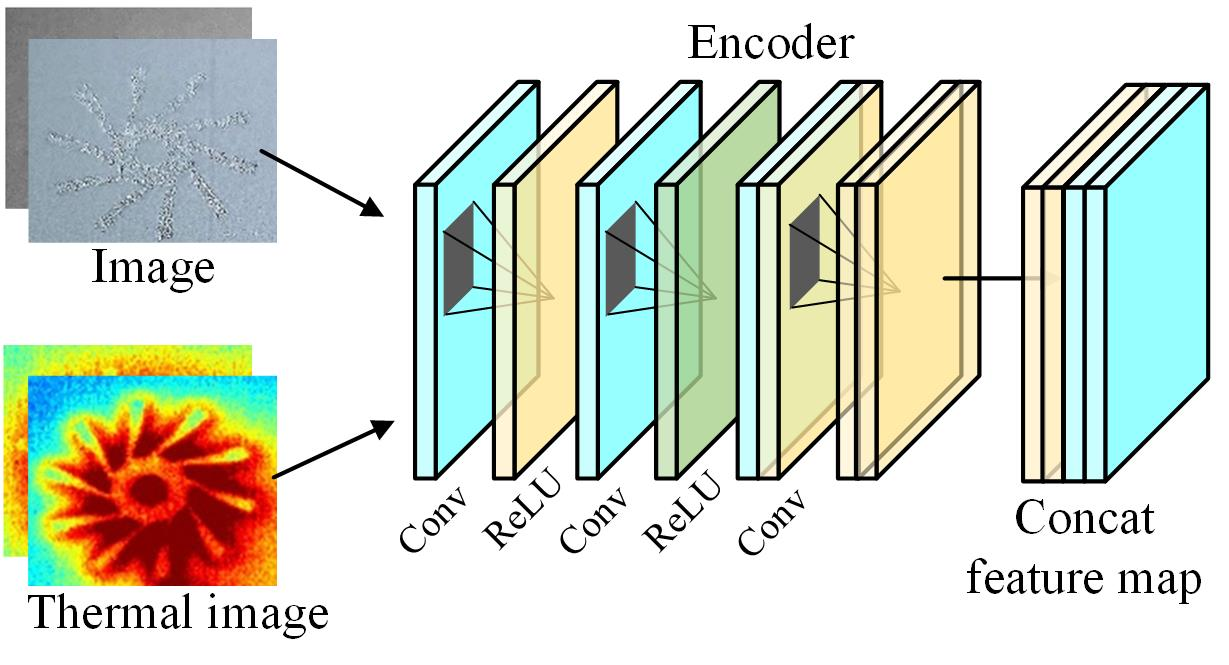
\includegraphics[width=0.4\textwidth]{fig2.jpg}
\caption{多模态特征提取模块}
\label{fig:feature_extractor}
\end{figure}

\subsection{因果一致性表征融合}

得到各模态的模态级向量后，若仅将其直接送入分类器，模型仍可能把特定工况下的亮度偏置、热场背景和纹理噪声一并编码为判别依据。因而，这里的关键并不在于构造更复杂的拼接结构，而在于在融合表示层显式约束跨工况稳定因素，使最终表征更多对应缺陷本身而非工况伴随信息。

具体而言，先将样本 $i$ 的多模态向量沿特征维拼接，形成统一输入
\begin{equation}
\mathbf{g}_i = \mathrm{Concat}\!\left(\mathbf{z}_i^{(m_1)}, \dots, \mathbf{z}_i^{(m_{K_i})}\right) \in \mathbb{R}^{K_i d_v}.
\label{eq:concat}
\end{equation}
其中，$\mathbf{g}_i$ 仅表示不同模态观测的联合描述。为将其映射到可施加一致性约束的统一融合空间，定义
\begin{equation}
\mathbf{h}_i = \phi_{\theta_f}\!\left(\mathrm{LN}(\mathbf{g}_i)\right) \in \mathbb{R}^{d_h}.
\label{eq:fusion}
\end{equation}
其中，$\mathrm{LN}(\cdot)$ 表示 LayerNorm，$d_h$ 为融合空间维度。融合头 $\phi_{\theta_f}$ 采用低参数的两层感知机实现，其职责仅限于完成跨模态特征压缩与重组；对工况伪相关的抑制并不依赖更深的融合网络，而是通过后续因果一致性约束直接作用于 $\mathbf{h}_i$。

因果一致性约束建立在如下假设之上：对于同一缺陷类别，不同工况下的背景纹理、亮度分布和热场响应可以发生变化，但决定类别归属的缺陷形态与异常热特征应保持稳定。为了使这一稳定因素在融合空间中显式可约束，本文首先对融合向量做 $\ell_2$ 归一化：
\begin{equation}
\bar{\mathbf{h}}_i = \frac{\mathbf{h}_i}{\|\mathbf{h}_i\|_2} \in \mathcal{S}^{d_h-1}.
\label{eq:norm}
\end{equation}
归一化后的 $\bar{\mathbf{h}}_i$ 仅保留方向信息，便于后续以余弦相似度刻画融合表征的跨工况一致性。与直接约束特征幅值相比，这种处理更关注不同样本在缺陷语义上的相对接近关系。

在此基础上，为每个样本构造同标签异工况的参照对象。对样本 $i$，定义其跨工况正样本池为
\begin{equation}
\Omega_i = \left\{ j \mid j \neq i,\; y_j = y_i,\; c_j \neq c_i \right\}.
\label{eq:pool}
\end{equation}
其中，$y_j = y_i$ 保证两者属于同一缺陷类别，$c_j \neq c_i$ 则强制二者来自不同工况。这样的配对方式避免模型仅在同工况样本之间学习表面相似性，而是要求同一缺陷类别在工况变化下仍保持接近的融合表征。应当指出，这里的因果一致性约束作用于样本 $i$ 与其同标签异工况正样本之间的融合表示，而非不同模态之间的直接对齐。若某个样本不存在可用的跨工况正样本，则该样本在当前 batch 中不参与一致性损失计算。

对于当前批量 $\mathcal{B}$ 中具有有效正样本的锚点集合 $\mathcal{B}^{+}=\{i\in\mathcal{B}\mid\Omega_i\neq\varnothing\}$，从 $\Omega_i$ 中选取一个正样本 $\pi(i)$，定义因果一致性损失为
\begin{equation}
\mathcal{L}_{\mathrm{cc}} =
\frac{1}{|\mathcal{B}^{+}|}
\sum_{i\in\mathcal{B}^{+}}
\left(
1-\bar{\mathbf{h}}_i^{\top}\sg\!\left(\bar{\mathbf{h}}_{\pi(i)}\right)
\right),
\label{eq:cc}
\end{equation}
其中，$\sg(\cdot)$ 表示梯度停止算子，用于阻断参照分支的梯度回传。由于 $\bar{\mathbf{h}}_i$ 和 $\bar{\mathbf{h}}_{\pi(i)}$ 已做归一化处理，二者内积可直接表征其余弦相似度，因此式~\eqref{eq:cc} 实质上是在拉近同标签异工况样本的融合表征，使一致的缺陷语义在不同工况下保持接近，并将工况差异排除在主要判别依据之外。

这一设计对应本文的方法假设：真正与标签稳定相关的应是缺陷形态、熔合状态和热异常模式本身，而不是某一特定设备或工艺条件带来的背景统计。因果一致性融合的作用，正是在多模态互补信息已经汇聚的基础上，通过同标签异工况对齐进一步剥离工况诱导的伪相关，从而为后续分类器提供跨工况更稳定的融合表示。

\begin{figure}[!t]
\centering
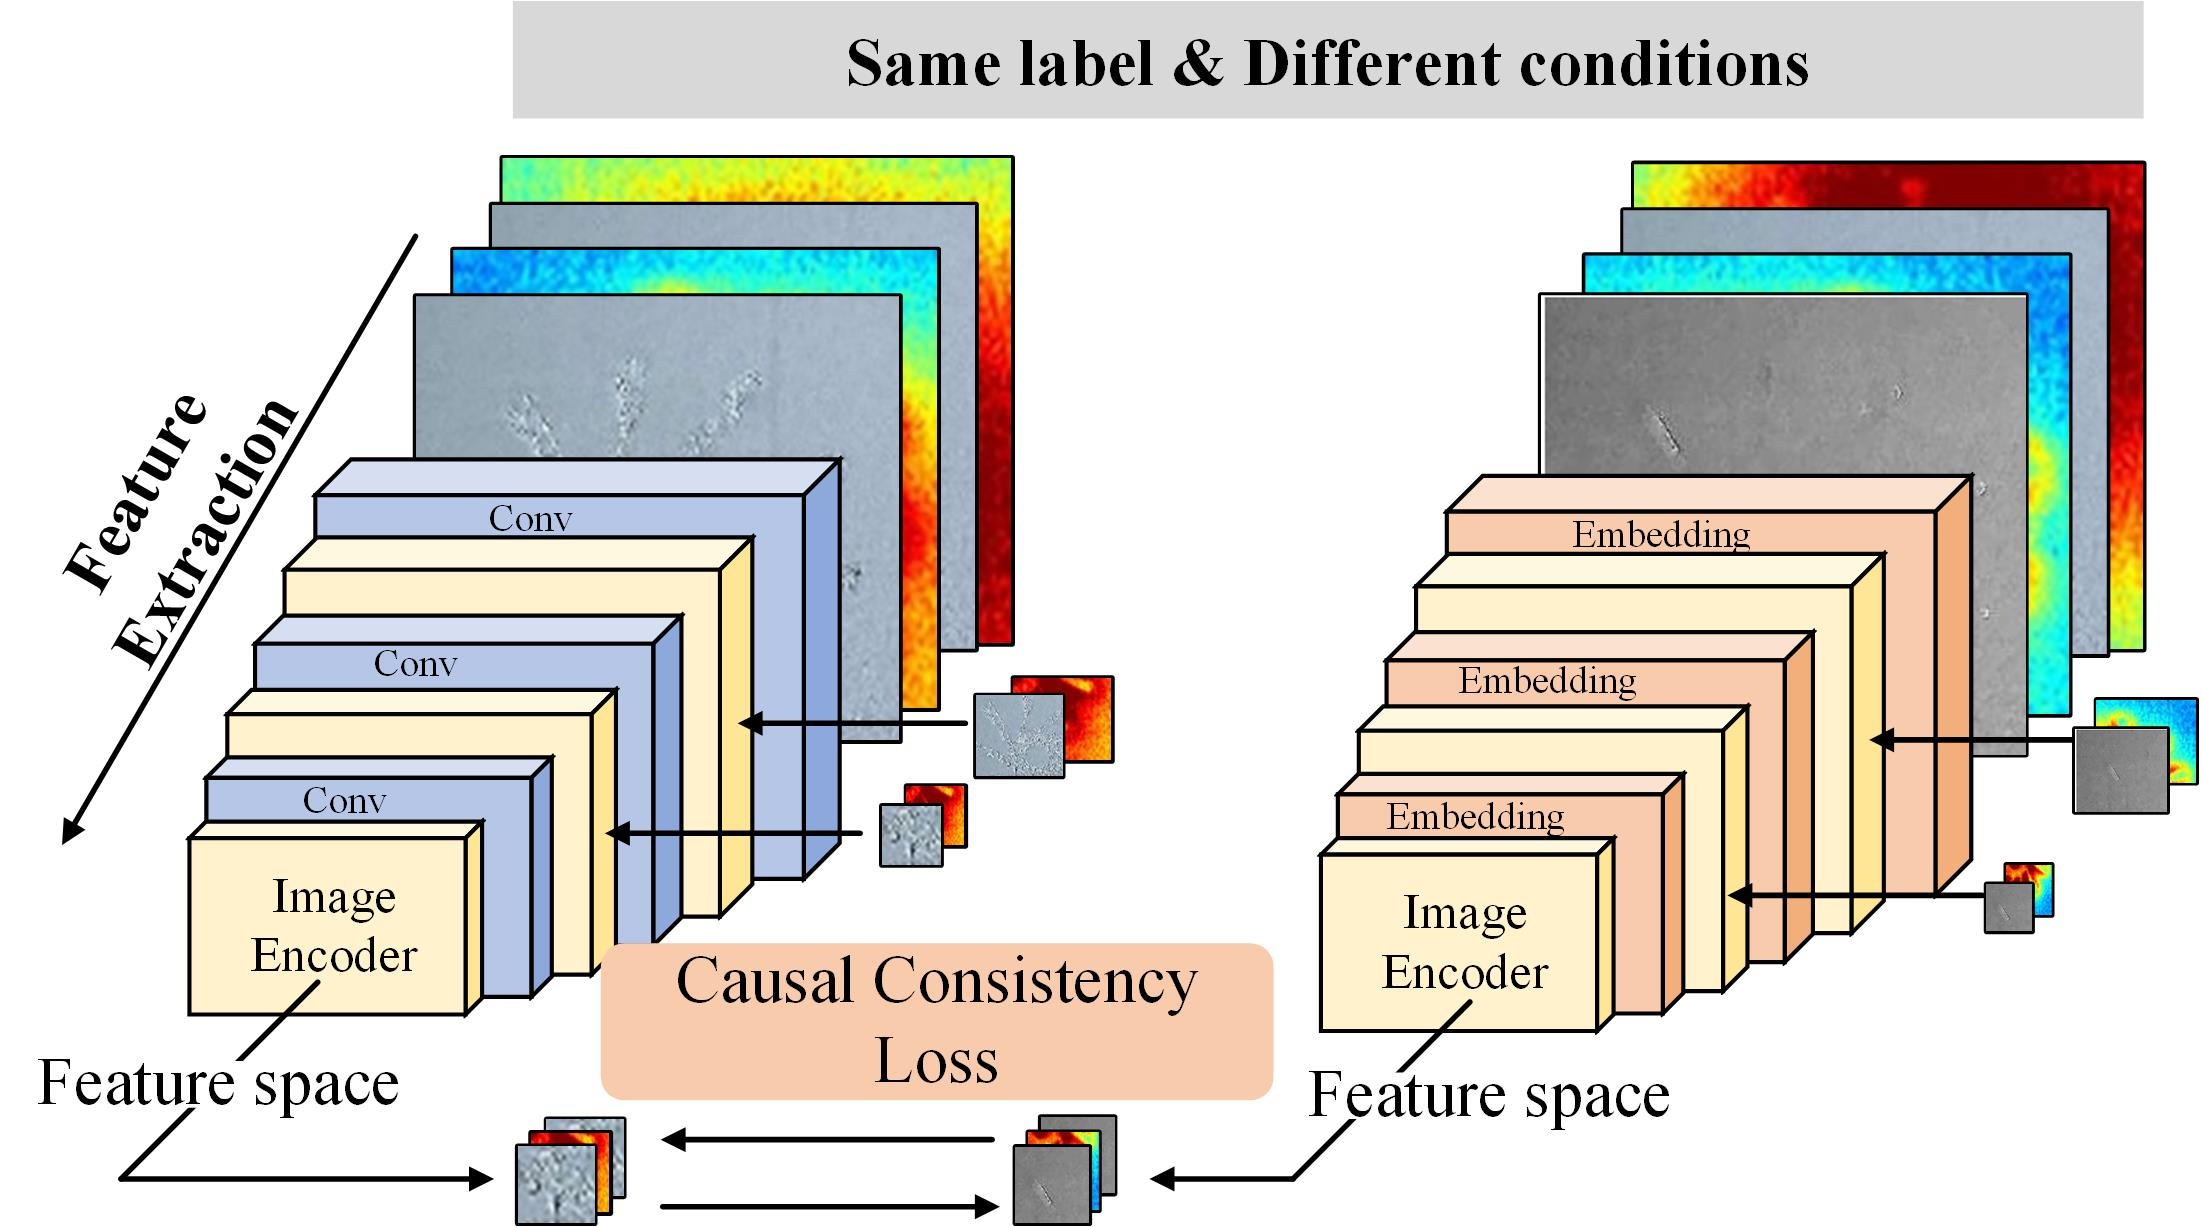
\includegraphics[width=0.45\textwidth]{fig3.jpg}
\caption{因果一致性融合模块}
\label{fig:causal_fusion}
\end{figure}

\subsection{基于大模型泛化先验的轻量适配}

在得到经过因果一致性约束的融合表示后，仍需进一步将预训练大模型在开放域视觉数据上形成的泛化先验迁移到未见工况缺陷识别任务中。若直接对整个视觉主干进行端到端微调，有限样本极易把这种泛化先验改写为少量工况样本上的局部经验；但若完全不进行任务适配，融合表示又难以形成与缺陷类别对应的稳定判别边界。因此，本文在冻结视觉主干的前提下，仅通过轻量融合头与分类头完成任务适配，以尽量保留大模型的泛化能力并提升未见工况下的识别性能。

具体地，利用上一节得到的融合向量 $\mathbf{h}_i$ 计算分类得分向量：
\begin{equation}
\boldsymbol{\ell}_i = \mathbf{W}_c \mathbf{h}_i + \mathbf{b}_c \in \mathbb{R}^{|\mathcal{Y}|},
\label{eq:scores}
\end{equation}
其中，$\mathbf{W}_c \in \mathbb{R}^{|\mathcal{Y}| \times d_h}$ 和 $\mathbf{b}_c \in \mathbb{R}^{|\mathcal{Y}|}$ 分别表示分类头的权重矩阵与偏置向量，$|\mathcal{Y}|$ 表示缺陷识别任务中的类别数。向量 $\boldsymbol{\ell}_i$ 的第 $k$ 个分量表示样本 $i$ 指向第 $k$ 类的未归一化判别得分。相应地，经 softmax 归一化后，样本 $i$ 属于各类别的预测概率为
\begin{equation}
\hat{\mathbf{y}}_i = \mathrm{softmax}(\boldsymbol{\ell}_i).
\label{eq:softmax}
\end{equation}
式中，$\hat{\mathbf{y}}_i$ 为三维概率向量，其第 $k$ 个分量表示样本属于第 $k$ 类的预测概率。分类器直接作用于未归一化的 $\mathbf{h}_i$，而归一化表示 $\bar{\mathbf{h}}_i$ 仅用于一致性约束，这一设置与实际训练代码完全一致。

基于式~\eqref{eq:softmax}，分类损失采用标准交叉熵形式：
\begin{equation}
\mathcal{L}_{\mathrm{cls}} = -\frac{1}{|\mathcal{B}|}\sum_{i \in \mathcal{B}} \log \hat{y}_{i,y_i},
\label{eq:ce}
\end{equation}
其中，$|\mathcal{B}|$ 表示 batch 大小，$\hat{y}_{i,y_i}$ 表示样本 $i$ 在真实标签 $y_i$ 上的预测概率。$\mathcal{L}_{\mathrm{cls}}$ 的作用是学习缺陷类别边界，而上一节的 $\mathcal{L}_{\mathrm{cc}}$ 则负责抑制工况诱导的表示漂移；二者分别对应类别可分性与跨工况稳定性两个目标。

在参数更新策略上，本文冻结预训练视觉编码主干，仅更新融合头参数 $\theta_f$ 与分类头参数 $\theta_c=(\mathbf{W}_c,\mathbf{b}_c)$。这种轻量适配方式将任务相关更新限制在小规模新增模块中，从而在有限标注条件下尽量保留大模型的泛化先验，避免未见工况识别过度依赖训练工况中的局部统计特征。

综合以上设计，模型的最终优化目标写为
\begin{equation}
\mathcal{L} = \mathcal{L}_{\mathrm{cls}} + \lambda \mathcal{L}_{\mathrm{cc}},
\label{eq:total}
\end{equation}
其中，$\lambda$ 为一致性约束权重，本文主实验取 $\lambda=0.1$。式~\eqref{eq:total} 表明，本文并非单纯追求训练集上的分类正确率，而是同时要求模型在融合空间中保持跨工况稳定，从而把大模型先验真正转化为未见工况下可用的判别能力。


\subsection{训练流程与整体架构}

训练阶段采用标准 mini-batch 梯度下降，但每一轮更新都依次经过共享视觉编码、多模态融合、因果一致性对齐和判别优化四个步骤。对 batch 中的每个样本，模型先按照当前模态组合组织输入观测，并由共享视觉主干提取模态级向量；随后通过融合头得到 $\mathbf{h}_i$ 和 $\bar{\mathbf{h}}_i$，分别用于分类损失与一致性损失计算。若当前 batch 中存在同标签异工况正样本，则额外计算 $\mathcal{L}_{\mathrm{cc}}$；否则仅优化 $\mathcal{L}_{\mathrm{cls}}$。主实验使用 AdamW 优化器与 cosine 学习率调度，在验证集上按 Macro-F1 选择最优 epoch，并配合 early stopping 控制过拟合。

表~\ref{tab:method_train_algo} 给出了 MCSQ-Net 的训练流程伪代码，表~\ref{tab:method_model_arch} 汇总了 MCSQ-Net 的关键结构配置。这两张表分别说明模型训练过程和核心组成，共同构成方法章的实现性描述。

\begin{table*}[!t]
\centering
\caption{MCSQ-Net 训练流程伪代码}
\label{tab:method_train_algo}
\footnotesize
\begin{tabular}{@{}p{0.97\textwidth}@{}}
\toprule
\textbf{训练流程} \\
\midrule
\begin{minipage}[t]{0.97\textwidth}
\begin{algorithmic}[1]
\STATE \textbf{输入：}训练集 $\mathcal{D}_{\mathrm{train}}$，验证集 $\mathcal{D}_{\mathrm{val}}$，共享视觉主干 $f_{\theta_v}$，融合头 $\phi_{\theta_f}$，分类头 $(\mathbf{W}_c,\mathbf{b}_c)$，权重系数 $\lambda$
\STATE \textbf{初始化：}冻结 $f_{\theta_v}$ 的全部视觉层；根据标签和 \texttt{condition\_uid} 为训练样本建立同标签异工况正样本池
\FOR{epoch $=1$ to $E$}
    \FOR{mini-batch $\mathcal{B}$}
        \STATE 按当前模态组合读取每个样本的输入观测，并送入共享视觉主干
        \STATE 对每个模态的空间特征序列做均值池化，得到模态级向量 $\mathbf{z}_i^{(m)}$
        \STATE 拼接所有模态向量，经融合头得到 $\mathbf{h}_i$ 及其归一化表示 $\bar{\mathbf{h}}_i$
        \STATE 由分类头计算分类得分，并得到分类损失 $\mathcal{L}_{\mathrm{cls}}$
        \IF{batch 中存在有效正样本对}
            \STATE 依据同标签异工况匹配关系计算一致性损失 $\mathcal{L}_{\mathrm{cc}}$
        \ELSE
            \STATE 令 $\mathcal{L}_{\mathrm{cc}} \leftarrow 0$
        \ENDIF
        \STATE 计算总损失 $\mathcal{L}=\mathcal{L}_{\mathrm{cls}}+\lambda \mathcal{L}_{\mathrm{cc}}$
        \STATE 反向传播并更新可训练参数
    \ENDFOR
    \STATE 在验证集上评估当前模型，并按主指标保存最优 checkpoint
    \IF{连续若干 epoch 未提升}
        \STATE 触发 early stopping
\ENDIF
\ENDFOR
\STATE \textbf{输出：}验证集最优的模型参数及其测试集评估结果
\end{algorithmic}
\end{minipage} \\
\bottomrule
\end{tabular}
\end{table*}

\begin{table*}[!t]
\centering
\caption{MCSQ-Net 的关键模型结构配置}
\label{tab:method_model_arch}
\footnotesize
\begin{tabular}{p{2.8cm}p{7.0cm}p{5.2cm}}
\toprule
模块 & 结构 & 作用 \\
\midrule
共享视觉主干 & 预训练视觉编码器，$d_v=1536$，冻结全部视觉层 & 提取统一模态特征 \\
模态级聚合 & 均值池化，$\mathbf{z}_i^{(m)}\in\mathbb{R}^{d_v}$ & 生成模态级表示 \\
输入组织 & 单视觉、单红外、视觉-红外组合输入 & 比较不同输入配置 \\
特征拼接 & $\mathbf{g}_i=\mathrm{Concat}(\mathbf{z}_i^{(m_1)},\dots,\mathbf{z}_i^{(m_{K_i})})\in\mathbb{R}^{K_i d_v}$ & 保留模态互补信息 \\
融合头 & $\mathrm{LN}+\mathrm{Linear}(K_i d_v,512)+\mathrm{GELU}+\mathrm{Dropout}(0.1)+\mathrm{Linear}(512,512)+\mathrm{GELU}$ & 压缩并重组融合特征 \\
一致性约束 & 同标签异工况配对，余弦一致性损失，$\lambda=0.1$ & 抑制工况诱导偏移 \\
分类头 & $\mathrm{Linear}(512,|\mathcal{Y}|)$ & 输出缺陷类别得分 \\
轻量适配 & 训练参数 $\{\theta_f,\theta_c\}$，batch size $=4$ & 保留大模型泛化先验 \\
\bottomrule
\end{tabular}
\end{table*}

\section{实验与分析}
\subsection{实验设置}
实验数据来源于自主搭建的开放式选择性激光熔化原位监测平台，如图~\ref{fig:platform_setup} 所示。平台采用 500~W 单模连续光纤激光器、振镜扫描系统和 PBAM 可编程控制软件，可对激光功率、扫描速度等关键工艺参数进行实时调整；成形过程在高纯氩气保护下进行，氧气体积分数控制在 0.1\% 以下。为采集多模态过程信号，平台配置两台 KM2010-3660 工业相机和一台 Optris PI 08M 短波红外热像仪，分别记录俯视/侧视可见光图像及垂直红外热场，并通过 TTL 外部触发实现帧级同步。基于该平台构建的数据集包含视觉模态、红外模态及对应工况信息，用于后续未见工况识别评估。

\begin{figure}[!t]
\centering
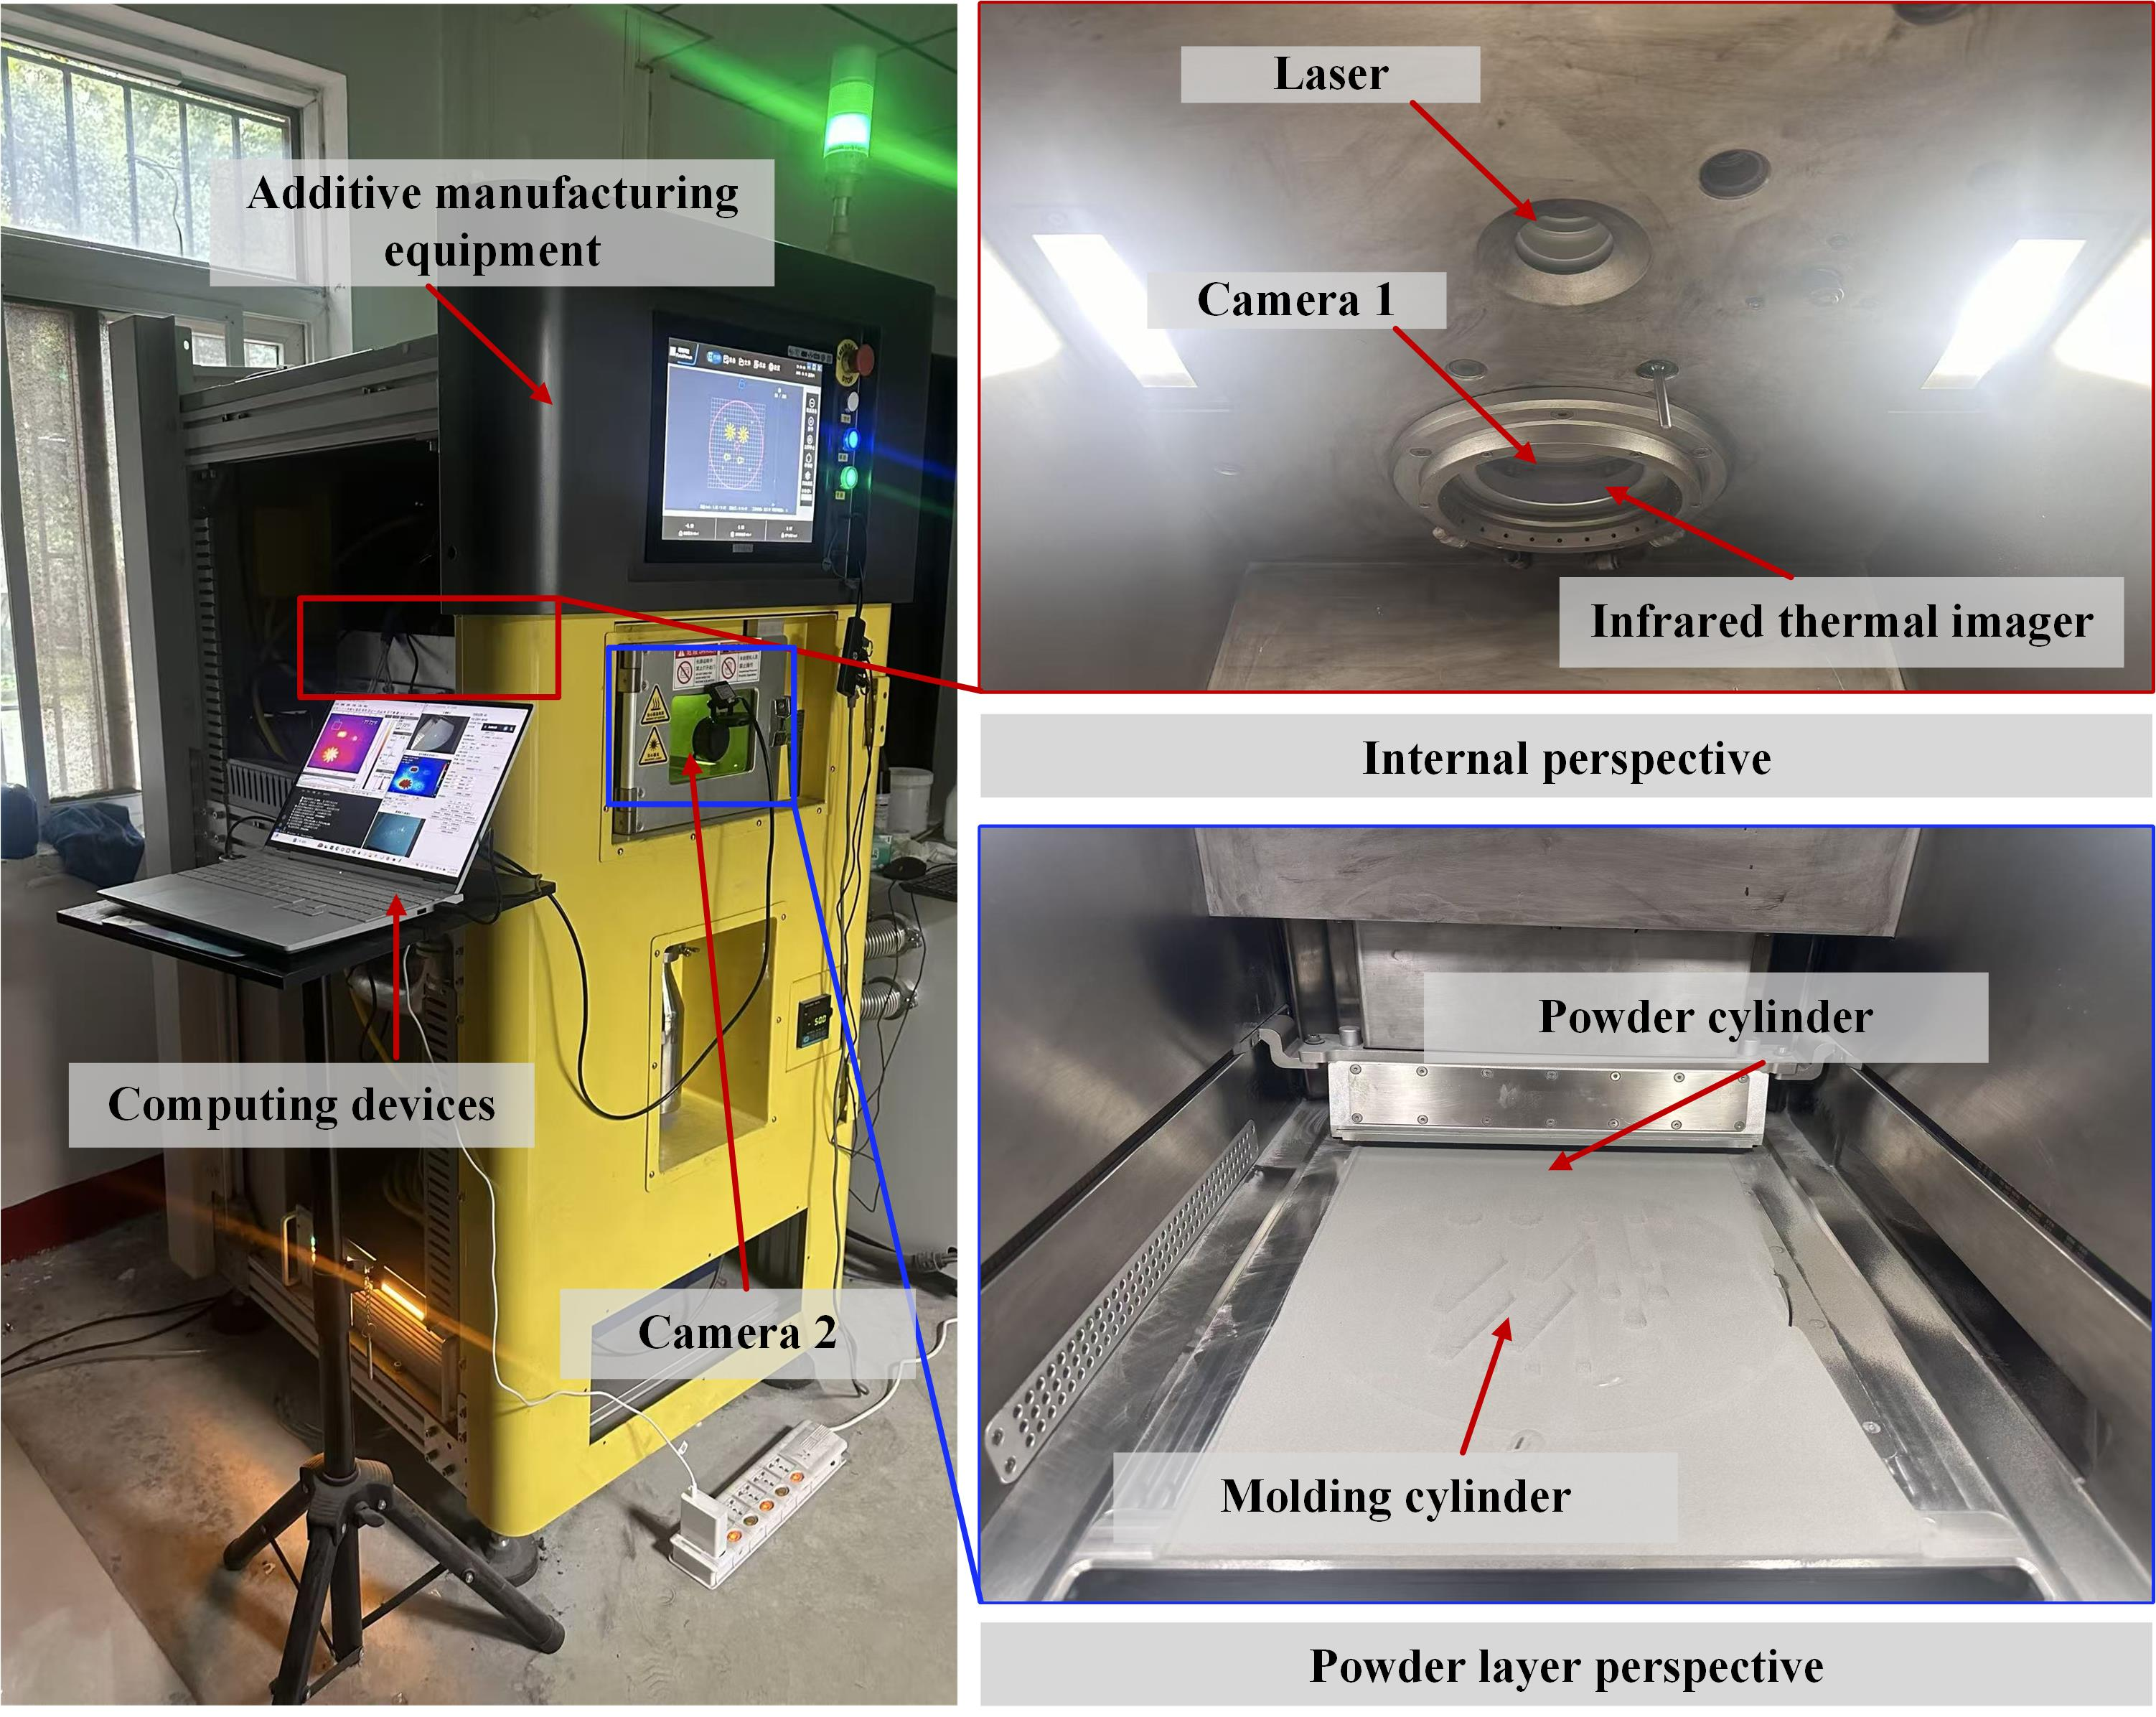
\includegraphics[width=0.45\textwidth]{fig4.jpg}
\caption{开放式 SLM 原位监测实验平台与多传感器数据采集系统占位图。定稿时将在此展示激光加工单元、控制系统以及双视觉-红外监测阵列。}
\label{fig:platform_setup}
\end{figure}

主方法采用 Qwen2-VL-2B-Instruct 的视觉编码主干，融合空间维度设为 512，dropout 为 0.1，batch size 为 4，优化器为 AdamW，学习率为 $3\times10^{-4}$，weight decay 为 $10^{-4}$，并使用 cosine 调度、混合精度训练与 patience 为 2 的 early stopping。在输入形式上，主方法比较了视觉模态、红外模态及其组合的识别效果，主实验采用性能最优的输入配置。实验中记录的工艺参数用于划分不同工况并构造同标签异工况正样本；类别标签仅作为监督信号参与训练，而不作为推理阶段的输入。因果稳定约束权重取 0.1。真微调对照实验使用 batch size 1、3 个 epoch、patience 为 1，视觉侧学习率为 $2\times10^{-6}$，融合头学习率为 $5\times10^{-5}$，梯度裁剪阈值为 0.5。最强经典基线为 ResNet18 + 双视觉输入 + MLP-concat。所有源域结果均在 3 个折上汇总，实验任务设置如表~\ref{tab:task_setup} 所示。

\begin{table*}[!t]
\centering
\caption{实验任务设置}
\label{tab:task_setup}
\footnotesize
\begin{tabular}{p{1.8cm}p{4.0cm}p{10.2cm}}
\toprule
编号 & 任务名称 & 任务设置 \\
\midrule
Task-1 & 源域未见工况缺陷类别识别 & 按工况划分三折交叉验证；训练、验证与测试集不共享相同工况；标签为健康（\texttt{normal}）、高功率翘曲（\texttt{HEW}）和低功率异常未熔合（\texttt{LEL}）；用于评估模型在未见工况下对具体缺陷类别的精细识别能力。 \\
Task-2 & 源域未见工况缺陷识别 & 沿用 Task-1 的工况划分；健康（\texttt{normal}）为正常类，其余两类缺陷合并为缺陷类（\texttt{abnormal}）；用于分析模型在未见工况下的异常识别能力，并为由闭集缺陷识别向开集异常识别拓展提供参考。 \\
Task-3 & 外部迁移缺陷类别识别 & 以 Task-1 的训练源域为基础，在独立外部测试集上评估；测试集不参与模型选择，用于检验跨设备、跨工艺条件下的识别稳定性。 \\
\bottomrule
\end{tabular}
\end{table*}

本文统一报告 Accuracy、Balanced Accuracy 和 Macro-F1 三项指标。Accuracy 反映总体分类正确率；Balanced Accuracy 取各类别召回率的平均值，可减弱类别分布不均衡对结果的影响；Macro-F1 对各类别 F1 值做无权平均，更能反映模型在不同缺陷类别上的整体识别均衡性。考虑到未见工况缺陷识别同时面临类别不均衡和跨类别性能波动，后文分析主要结合 Balanced Accuracy 与 Macro-F1 展开。

\subsection{未见工况下的缺陷识别}
Task-1 直接对应本文关注的未见工况缺陷类别识别任务，因此也是全文最主要的实验。围绕该任务，本文系统比较了三类路线：其一为 Prompt-Qwen 闭集分类基线；其二为经典判别式 CNN 基线，包括单相机输入、红外单模态输入、双相机 MLP 拼接、跨注意力融合以及三模态晚期融合等结构；其三为本文提出的 MCSQ-Net 及其主要变体。表~\ref{tab:data1_main_cn} 汇报了主任务中的主要对比结果。可以看出，Prompt-Qwen 仅取得 0.3914 的 Macro-F1，说明直接 prompt 适配并不能有效利用大模型先验；经典 CNN 路线中，当前最优结果由 ResNet18 + Camera 1 \& 2 + MLP-concat 取得，Macro-F1 为 0.8323；MCSQ-Net 则进一步将 Macro-F1 提升至 0.8547。由此可见，真正有效的并非简单扩大模型规模，而是在保留大模型泛化先验的基础上，通过显式多模态融合与跨工况稳定约束提升判别表示质量。

\begin{table*}[!t]
\caption{Task-1 未见工况缺陷类别识别主结果}
\label{tab:data1_main_cn}
\centering
\begin{tabular}{|l|l|c|c|c|}
\hline
方法家族 & 具体设置 & Accuracy & Balanced Accuracy & Macro-F1 \\
\hline
Prompt-Qwen & 3-class prompt baseline & 0.4809 $\pm$ 0.0602 & 0.5021 $\pm$ 0.0460 & 0.3914 $\pm$ 0.0587 \\
\hline
Classic CNN & ResNet18 + Camera 1 \& 2 + MLP-concat（经典最优） & 0.8349 $\pm$ 0.0858 & 0.8412 $\pm$ 0.0846 & 0.8323 $\pm$ 0.0892 \\
\hline
MCSQ-Net & 完整模型 & \textbf{0.8521 $\pm$ 0.0929} & \textbf{0.8556 $\pm$ 0.0973} & \textbf{0.8547 $\pm$ 0.0955} \\
\hline
\end{tabular}
\end{table*}

Task-2 的二分类结果也支持同样结论。Prompt-Qwen 的二分类 Macro-F1 仅为 0.3903，MCSQ-Net 为 0.4707，均显著弱于经典最优二分类基线。因此，本文仍将缺陷类别识别作为主任务，而将该二分类结果主要用于分析模型在未见工况下的异常识别能力，并为后续向开集异常识别拓展提供实验参考。

\begin{figure}[!t]
\centering
% TODO: 替换为正式主结果图。
\fbox{\rule{0pt}{1.4in}\rule{0.95\columnwidth}{0pt}}
\caption{Task-1 未见工况缺陷类别识别结果占位图。}
\label{fig:data1_main_cn}
\end{figure}

除源域主任务外，本文进一步在 Task-3 上检验模型在更强复合分布偏移下的稳健性。表~\ref{tab:data2_transfer_cn} 展示了外部迁移测试中的最佳结果。Prompt-Qwen 的 Macro-F1 为 0.4073，经典最优迁移基线为 0.4236，而 MCSQ-Net 达到 0.6067。由于 Task-3 同时包含跨设备、跨工艺参数和复合分布偏移，因此这一结果说明，MCSQ-Net 的优势并不局限于源域工况划分下的闭集识别，也能延续到更困难的外部迁移场景。

\begin{table}[!t]
\caption{Task-3 外部迁移缺陷类别识别结果}
\label{tab:data2_transfer_cn}
\centering
\resizebox{\columnwidth}{!}{
\begin{tabular}{|l|c|c|}
\hline
家族 / 最佳模型 & Balanced Accuracy & Macro-F1 \\
\hline
Prompt-Qwen / \texttt{data1\_official\_cv\_3class\_baseline} & 0.4586 $\pm$ 0.0286 & 0.4073 $\pm$ 0.0511 \\
\hline
Classic / 三模态晚期融合 & 0.4973 $\pm$ 0.0954 & 0.4236 $\pm$ 0.1110 \\
\hline
MCSQ-Net / 双视觉输入 + 因果稳定约束 & \textbf{0.6359 $\pm$ 0.0158} & \textbf{0.6067 $\pm$ 0.0351} \\
\hline
\end{tabular}
}
\end{table}

迁移结果也进一步补全了本文的多模态叙事。红外信息在增材制造监测中依然具有物理意义和统计价值 \cite{ref_lpbf_sensing_review,ref_intelligent_defect_pbf}。当前 MCSQ-Net 的最优配置为 Camera 1 \& 2，主要反映的是现有融合结构和样本规模的约束，而不是 IR 在缺陷识别中没有作用。

\begin{figure}[!t]
\centering
% TODO: 替换为正式迁移结果图。
\fbox{\rule{0pt}{1.4in}\rule{0.95\columnwidth}{0pt}}
\caption{Task-3 外部迁移缺陷类别识别结果占位图。}
\label{fig:data2_transfer_cn}
\end{figure}

\subsection{消融实验}
为进一步说明 MCSQ-Net 的性能来源，本节从多模态组合和方法组成两个方面开展消融分析。表~\ref{tab:ablation_cn} 给出了多模态消融结果。可以看出，各模态均能提供有效缺陷信息，但其增益依赖具体融合方式。首先，IR only 仍能达到 0.6270 的 Macro-F1，说明红外热信息确实包含有意义的缺陷线索。其次，Camera 1 \& 2 是当前最稳定的输入配置，因为两个视角提供了更稳健的几何与纹理互补。最后，Camera 1 \& 2 + IR 没有超过 Camera 1 \& 2，说明当前问题不在于是否引入红外模态，而在于如何更有效地建模其热特征贡献。

\begin{table}[!t]
\caption{MCSQ-Net 多模态消融}
\label{tab:ablation_cn}
\centering
\begin{tabular}{|l|c|c|}
\hline
输入方式 & Balanced Accuracy & Macro-F1 \\
\hline
Camera 1 baseline & 0.7714 $\pm$ 0.0771 & 0.7419 $\pm$ 0.1203 \\
\hline
IR only & 0.6508 $\pm$ 0.0708 & 0.6270 $\pm$ 0.0878 \\
\hline
Camera 1 \& 2 & 0.8422 $\pm$ 0.1061 & 0.8402 $\pm$ 0.1048 \\
\hline
Camera 1 \& 2 + IR & 0.8169 $\pm$ 0.0659 & 0.8121 $\pm$ 0.0615 \\
\hline
Camera 1 \& 2 + 因果稳定约束 & \textbf{0.8556 $\pm$ 0.0973} & \textbf{0.8547 $\pm$ 0.0955} \\
\hline
\end{tabular}
\end{table}

这一判断与迁移基线的表现是相互印证的：在 Task-3 上，经典最优方法反而采用了三模态晚期融合。这进一步说明 IR 并非无效，而是其最佳利用方式与模型家族密切相关。

\begin{table}[!t]
\caption{MCSQ-Net 方法消融}
\label{tab:method_ablation_cn}
\centering
\begin{tabular}{|l|c|c|}
\hline
方法设置 & Balanced Accuracy & Macro-F1 \\
\hline
去除因果稳定约束 & 0.8422 $\pm$ 0.1061 & 0.8402 $\pm$ 0.1048 \\
\hline
完整模型 & \textbf{0.8556 $\pm$ 0.0973} & \textbf{0.8547 $\pm$ 0.0955} \\
\hline
解冻最后两个视觉块 & 0.7979 $\pm$ 0.0332 & 0.7781 $\pm$ 0.0411 \\
\hline
\end{tabular}
\end{table}

表~\ref{tab:method_ablation_cn} 进一步给出了方法消融结果。与去除因果稳定约束的版本相比，完整模型将 Macro-F1 从 0.8402 提升到 0.8547，将 Balanced Accuracy 从 0.8422 提升到 0.8556，说明在冻结式大模型融合框架已经成立的前提下，跨工况同标签对齐仍能进一步抑制工况诱导的伪相关。相反，若解冻最后两个视觉块，Macro-F1 会降至 0.7781，且在 Task-3 上也会从 0.6067 下降到 0.5808。该结果表明，当前问题并不是大模型先验“适配得还不够”，而是激进微调会破坏原有稳定视觉表征，引发对有限样本和工况特征的过拟合。因此，因果稳定约束的价值在于提升轻量适配的表示质量，而不是为激进真微调兜底。

\section{结论}
本文围绕一个更贴近工业部署的问题展开研究。在按工况划分训练与测试的交叉验证实验和更强外部迁移压力下，如何利用大模型先验实现金属增材制造多模态缺陷的稳定识别，是本文关注的核心。基于仓库正式实验结果，本文表明直接 Prompt-Qwen 路线并不适合当前小样本未见工况任务。相比之下，将 Qwen2-VL 作为视觉先验编码器，结合显式多模态融合与因果稳定约束，能够在源域交叉验证和外部迁移测试中同时取得最优表现。进一步地，真微调实验说明，当前更有效的路径不是继续激进解冻视觉主干，而是保留强先验、通过因果稳定约束提升表示质量。后续工作可进一步探索面向 IR 热特征的更细粒度融合机制，以及比直接解冻更温和的视觉侧 adapter/LoRA 方案。

\begin{thebibliography}{00}

\bibitem{ref_defect_formation_slm}
B.~Zhang, Y.~Li, and Q.~Bai, ``Defect formation mechanisms in selective laser melting: A review,'' \emph{Chinese Journal of Mechanical Engineering}, vol.~30, pp.~515--527, 2017.

\bibitem{ref_in_situ_monitoring_review}
X.~Peng, L.~Kong, H.~An, and G.~Dong, ``A review of in situ defect detection and monitoring technologies in selective laser melting,'' \emph{3D Printing and Additive Manufacturing}, vol.~10, no.~3, pp.~438--466, 2023.

\bibitem{ref_lpbf_sensing_review}
D.~Guillen, S.~Wahlquist, and A.~Ali, ``Critical review of LPBF metal print defects detection: Roles of selective sensing technology,'' \emph{Applied Sciences}, vol.~14, no.~15, p.~6718, 2024.

\bibitem{ref_intelligent_defect_pbf}
P.~Wang \emph{et al.}, ``Towards intelligent defect detection in metal powder bed fusion: A review of in situ monitoring, data pre-processing, and machine learning,'' \emph{Materials Science and Engineering: R: Reports}, vol.~167, p.~101112, 2026.

\bibitem{ref_anomalygpt}
Z.~Gu \emph{et al.}, ``AnomalyGPT: Detecting industrial anomalies using large vision-language models,'' arXiv:2308.15366, 2023.

\bibitem{ref_myriad}
Y.~Li \emph{et al.}, ``Myriad: Large multimodal model by applying vision experts for industrial anomaly detection,'' arXiv:2310.19070, 2023.

\bibitem{ref_vlm_active_learning}
S.~Chen and Y.~Liu, ``Vision-language model-assisted active learning for high-accuracy defect detection in automotive bushing components,'' in \emph{Proc. Int. Conf. Embodied Intelligence and Large Models}, 2025, pp.~9--14.

\bibitem{ref_qlora_excavator}
H.~V.~Nguyen, H.~Park, N.~Yoo, and J.~Yang, ``Resource-efficient fine-tuning of large vision-language models for multimodal perception in autonomous excavators,'' \emph{Frontiers in Artificial Intelligence}, vol.~8, p.~1681277, 2025.

\bibitem{ref_omniad}
S.~Zhao \emph{et al.}, ``OmniAD: Detect and understand industrial anomaly via multimodal reasoning,'' arXiv:2505.22039, 2025.

\bibitem{ref_ad_copilot}
X.~Jiang \emph{et al.}, ``AD-Copilot: A vision-language assistant for industrial anomaly detection via visual in-context comparison,'' arXiv:2603.13779, 2026.

\bibitem{ref_wu2024_multisensor}
Q.~Wu \emph{et al.}, ``In-situ quality intelligent classification of additively manufactured parts using a multi-sensor fusion based melt pool monitoring system,'' \emph{Additive Manufacturing Frontiers}, vol.~3, no.~3, p.~200153, 2024.

\bibitem{ref_liu2024_acoustic}
H.~Liu \emph{et al.}, ``Inference of highly time-resolved melt pool visual characteristics and spatially-dependent lack-of-fusion defects in laser powder bed fusion using acoustic and thermal emission data,'' \emph{Additive Manufacturing}, vol.~83, p.~104057, 2024.

\bibitem{ref_shen2024_multisource}
T.~Shen \emph{et al.}, ``Multi-source information fusion for enhanced in-process quality monitoring of laser powder bed fusion additive manufacturing,'' \emph{Additive Manufacturing}, vol.~96, p.~104575, 2024.

\bibitem{ref_li2024_transfer}
J.~Li \emph{et al.}, ``Transfer learning-based quality monitoring of laser powder bed fusion across materials,'' \emph{Expert Systems with Applications}, vol.~252, p.~124150, 2024.

\end{thebibliography}

\end{document}
